\chapter{Analysis}

\section {Actors}
\begin{itemize}
    \item \textbf{Unregistered User}: A visitor who has not created an account on the platform. They can browse media contents, search and filter, view media content details, and register/login.
    \item \textbf{Registered User}: A user who has created an account on the platform. They can perform all the actions of an unregistered user, as well as logout, manage their profile, explore other user profiles, interact with media contents/users, review media contents, and receive advanced recommendations.
    \item \textbf{Manager}: A registered user with administrative features. They can access an analytics dashboard, manage user accounts, content entries, and monitor trends.
\end{itemize}

\section{Requirements}
\textbf{Unregistered User}:

\begin{itemize}
    \item Browse Media Contents:
    \begin{itemize}
        \item View a list of available manga and anime on the home page.
        \item Access basic details about each media content without logging in.
    \end{itemize}
    \item Search and Filter:
    \begin{itemize}
        \item Use the search bar to find specific manga or anime by title.
        \item Utilize basic filtering options to refine the media content list.
    \end{itemize}
    \item View Media Content Details:
    \begin{itemize}
        \item Click on a media content to view detailed information, including synopsis and genre.
    \end{itemize}
    \item Register/Login:
    \begin{itemize}
        \item Access a registration page to create a new account.
        \item Use valid credentials to log into the account.
    \end{itemize}
    \item Explore Features:
    \begin{itemize}
        \item Access information about the features available to registered users.
    \end{itemize}
\end{itemize}

\textbf{Registered User}:

\begin{itemize}
    \item Browse Media Contents:
    \begin{itemize}
        \item View a list of available manga and anime on the home page.
        \item Access basic details about each media content without logging in.
    \end{itemize}
    \item Search and Filter:
    \begin{itemize}
        \item Use the search bar to find specific media content by title.
        \item Utilize basic filtering options to refine the media content list.
    \end{itemize}
    \item View Media Content Details:
    \begin{itemize}
        \item Click on a media content to view detailed information, including synopsis and genre.
    \end{itemize}
    \item Logout:
    \begin{itemize}
        \item Ends the user's session.
    \end{itemize}
    \item Profile Management:
    \begin{itemize}
        \item Edit and update personal information (e.g., profile picture, bio).
        \item Change account password.
    \end{itemize}
    \item Explore Other User Profiles:
    \begin{itemize}
        \item View profiles of other registered users.
        \item See their liked manga, anime and reviews.
    \end{itemize}
    \item Interact with Media Contents/Users:
    \begin{itemize}
        \item Like or dislike manga and anime to indicate preferences.
        \item Follow/unfollow other users.
    \end{itemize}
    \item Review Media Contents:
    \begin{itemize}
        \item Add reviews and ratings to manga and anime.
        \item View and edit own reviews.
    \end{itemize}
    \item Advanced Recommendations:
    \begin{itemize}
        \item Receive more refined media content suggestions based on detailed user interactions.
        \item Receive users suggestions based on common interests.
    \end{itemize}
\end{itemize}

\textbf{Manager}(Registered User with Administrative Features):

\begin{itemize}
    \item Analytics Dashboard:
    \begin{itemize}
        \item Access a comprehensive analytics dashboard with data on user engagement and media contents trends.
    \end{itemize}
    \item User Management:
    \begin{itemize}
        \item View and manage user accounts, including account activation and deactivation.
    \end{itemize}
    \item Content Management:
    \begin{itemize}
        \item Manage media content entries, including adding new manga and anime, updating information, and removing entries if necessary.
    \end{itemize}
    \item Monitor Trends:
    \begin{itemize}
        \item Monitor trends in user interactions, popular genres, and trending manga.
    \end{itemize}
\end{itemize}

\section{Non Functional Requirements}

\textbf{Performance}

\begin{itemize}
    \item Response Time: The system should have low latency, with pages loading within an acceptable timeframe.
    \item Scalability: The system should be able to handle an increasing number of users and data without significant degradation in performance.
    \item Concurrency: The application should support multiple users simultaneously without performance bottlenecks. For very high traffic scenarios, acceptable delays may be introduced.
\end{itemize}

\textbf{Security}

\begin{itemize}
    \item Data Encryption: All user data, including passwords, should be securely encrypted during transmission and storage.
\end{itemize}

\textbf{User Interface}

\begin{itemize}
    \item Responsiveness: The user interface should be responsive, providing a consistent and seamless experience across various devices and screen sizes.
    \item Intuitiveness: The interface should be user-friendly, with clear navigation and easily understandable features.
\end{itemize}

\section{UML use case diagram}
\begin{figure}[h]
    \centering
    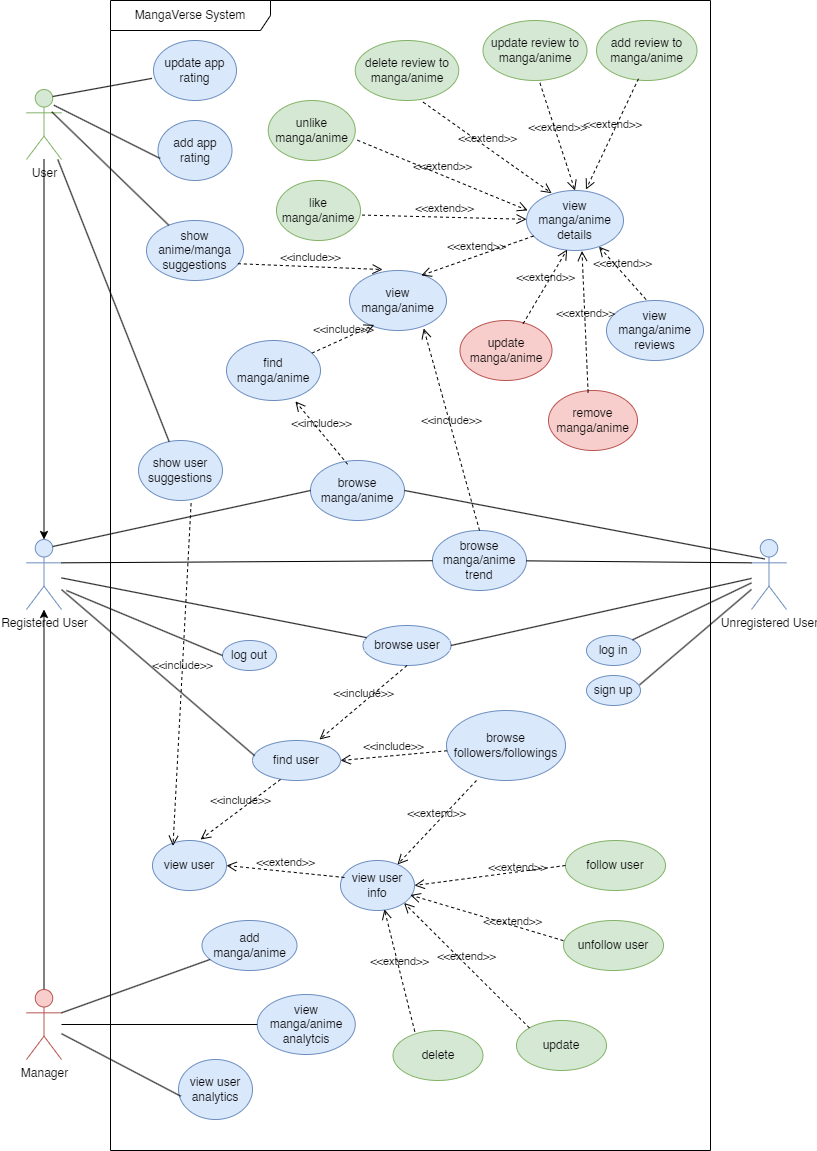
\includegraphics[width=\linewidth]{Media/use_case.png}
    \caption{UML Class Diagram}
    \label{uml class diagram}
\end{figure}

\newpage

\section{UML class diagram}
\begin{figure}[h]
    \centering
    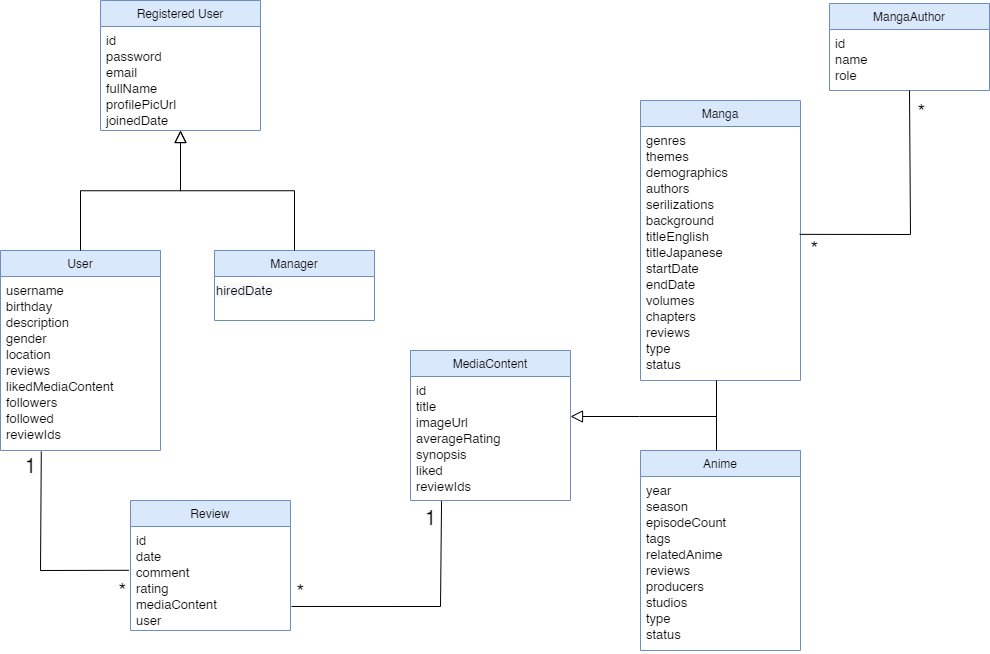
\includegraphics[width=\linewidth]{Media/Class_Diagram.png}
    \caption{UML Class Diagram}
    \label{uml class diagram}
\end{figure}

\newpage


\section{Data Modeling}
\subsection{Data Collection}
\textit{Sources:} https://www.kaggle.com/datasets/dbdmobile/myanimelist-dataset?select=users-score-2023.csv, MyAnimeList.net,	anilist.com,  kitsu.io,			  livechart.me,
anime-planet.com,		nofity.moe,	   anisearch.com,		  anidb.net 	

\textit{Description:} Manga, users and scores datasets were collected from MyAnimeList.net site using the official API and another unofficial API (Jikan). The anime datasets were collected from all the sources. 

\textit{Variety:} The datasets contain a variety of data types, including text, numbers, and dates. Anime are collected from 8 different sources. All the information is collected in 4 different csv files.

\textit{Volume:} The datasets contain a large volume of data, with thousands of entries for anime, manga, users, and scores. The total size of the datasets is around 3 GB.

\subsection{Data Cleaning and Preprocessing}
Python scripts were used to clean and preprocess the data. The following steps were performed:
reviews were created by merging the users and scores datasets, and creating comments about the media contents;
the anime dataset was created by putting togethere the diffrerent sources;
the manga dataset was created from MyAnimeList.net;
the users dataset was cleaned and missing information, like email and password, was added.

